% Generated by gen_figs.py from the reform tables (FROT 2025 simulation). Each point is one reform:
% x = net fiscal cost (% change in NPV of government spending), y = WTP (consumption-equivalent welfare change, %).
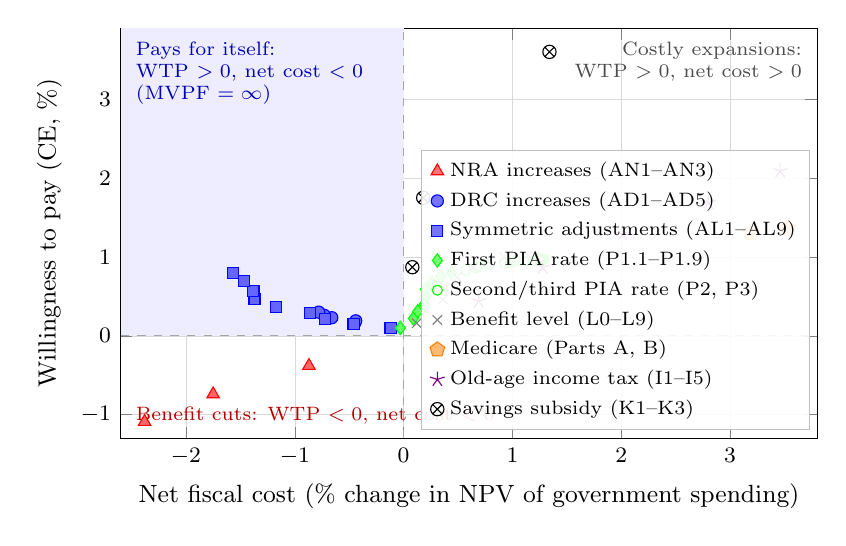
\begin{tikzpicture}
\begin{axis}[width=0.86\textwidth,height=0.56\textwidth,
  xmin=-2.6,xmax=3.8,ymin=-1.3,ymax=3.9,
  xlabel={Net fiscal cost (\% change in NPV of government spending)},
  ylabel={Willingness to pay (CE, \%)},
  grid=both,grid style={line width=.1pt, draw=gray!15},major grid style={line width=.2pt,draw=gray!30},
  tick label style={font=\footnotesize},label style={font=\small},
  legend style={font=\scriptsize,at={(0.99,0.02)},anchor=south east,draw=gray!50,fill=white,fill opacity=0.9,text opacity=1,cells={anchor=west}},
  legend cell align=left]
\fill[blue!7] (axis cs:-2.6,0) rectangle (axis cs:0,3.9);
\draw[gray!70,dashed] (axis cs:-2.6,0) -- (axis cs:3.8,0);
\draw[gray!70,dashed] (axis cs:0,-1.3) -- (axis cs:0,3.9);
\node[font=\scriptsize,align=left,anchor=north west,text=blue!70!black] at (axis cs:-2.55,3.85) {Pays for itself:\\ WTP $>0$, net cost $<0$\\ (MVPF $=\infty$)};
\node[font=\scriptsize,align=right,anchor=north east,text=black!70] at (axis cs:3.75,3.85) {Costly expansions:\\ WTP $>0$, net cost $>0$};
\node[font=\scriptsize,align=left,anchor=south west,text=red!70!black] at (axis cs:-2.55,-1.25) {Benefit cuts: WTP $<0$, net cost $<0$};
\addplot[only marks,mark=triangle*,mark size=2.6pt,color=red,mark options={solid,fill=red!60,draw=red}] coordinates {(-0.87,-0.38) (-1.75,-0.74) (-2.38,-1.09)};
\addlegendentry{NRA increases (AN1--AN3)}
\addplot[only marks,mark=*,mark size=2.2pt,color=blue,mark options={solid,fill=blue!60,draw=blue}] coordinates {(-0.45,0.16) (-0.44,0.19) (-0.66,0.23) (-0.73,0.26) (-0.78,0.3)};
\addlegendentry{DRC increases (AD1--AD5)}
\addplot[only marks,mark=square*,mark size=2.0pt,color=blue,mark options={solid,fill=blue!60,draw=blue}] coordinates {(-0.12,0.1) (-0.46,0.15) (-0.72,0.21) (-0.86,0.29) (-1.17,0.37) (-1.37,0.47) (-1.38,0.57) (-1.47,0.69) (-1.57,0.8)};
\addlegendentry{Symmetric adjustments (AL1--AL9)}
\addplot[only marks,mark=diamond*,mark size=2.4pt,color=green,mark options={solid,fill=green!60,draw=green}] coordinates {(-0.03,0.1) (0.09,0.22) (0.13,0.31) (0.19,0.4) (0.21,0.5) (0.2,0.59) (0.26,0.67) (0.34,0.75) (0.44,0.8)};
\addlegendentry{First PIA rate (P1.1--P1.9)}
\addplot[only marks,mark=o,mark size=1.8pt,color=green,mark options={solid,fill=green!60,draw=green}] coordinates {(0.57,0.83) (0.67,0.86) (0.7,0.88) (0.78,0.9) (0.93,0.92) (0.98,0.93) (1.03,0.95) (1.11,0.94) (1.19,0.95) (1.27,0.95) (1.26,0.95) (1.27,0.96) (1.28,0.96) (1.26,0.96) (1.27,0.96) (1.29,0.97) (1.27,0.97) (1.27,0.97) (1.25,0.97) (1.24,0.98)};
\addlegendentry{Second/third PIA rate (P2, P3)}
\addplot[only marks,mark=x,mark size=2.4pt,color=gray,mark options={solid,fill=gray!60,draw=gray}] coordinates {(0.12,0.16) (0.21,0.32) (0.36,0.46) (0.38,0.6) (0.49,0.74) (0.64,0.87) (0.79,0.95) (0.92,1) (1.14,1.02) (1.24,0.98)};
\addlegendentry{Benefit level (L0--L9)}
\addplot[only marks,mark=pentagon*,mark size=2.8pt,color=orange,mark options={solid,fill=orange!60,draw=orange}] coordinates {(3.53,1.36) (3.19,1.3)};
\addlegendentry{Medicare (Parts A, B)}
\addplot[only marks,mark=star,mark size=2.8pt,color=violet,mark options={solid,fill=violet!60,draw=violet}] coordinates {(0.69,0.44) (1.28,0.87) (2.01,1.29) (2.8,1.69) (3.46,2.09)};
\addlegendentry{Old-age income tax (I1--I5)}
\addplot[only marks,mark=otimes,mark size=2.4pt,color=black,mark options={solid,fill=black!60,draw=black}] coordinates {(0.08,0.87) (0.18,1.75) (1.34,3.6)};
\addlegendentry{Savings subsidy (K1--K3)}
\end{axis}
\end{tikzpicture}
